% 格式与内容分离是Latex的基本思想
% -----------------------导言区-------------------------
%\documentclass{article} % book, report, letter 
% 对于ctex, 有ctexart, ctexrep, ctexbook文档类, 使用这三个文档类时,不需要再使用\usepackage{ctex}命令导入ctex宏包。
% \documentclass{ctexart}
\documentclass[12pt]{article} % Normal Size字体大小, 只有10-12三个设置

\usepackage{ctex}
\usepackage{graphicx}
\usepackage{amsmath}
\usepackage{amssymb}

% ================= bibtex
% \usepackage{netbib}
% netbib提供更多的样式 plainnet 
% \bibliographystyle{plain}
% \bibliographystyle[round]{plain}	\cite \citep
% 清华北大等提供了很多中文常用的样式
% 参考文献可以通过jabref等软件辅助处理

% \bibliographystyle{plain} % 排版样式 : plain unsrt alpha abbrv

% ================= biblatex
% caspervector 是符合国标的陪伴文件
% \usepackage[style=numeric,backend=biber]{biblatex}
% 排序需要设置参数biber.exe -l zh__pinyin %  
\usepackage[style=caspervector, backend=biber, utf8, sorting=centy]{biblatex} % 排序的先后顺序, c - 中文 e - 英文 n - 姓名 t - 标题 y - 年份。 需要两次编译。
\addbibresource{example.bib}


% 可以用 \ctexset 命令对段落进行设置 ,必须使用ctex的文档类
% 详见 texdoc ctex
\if false		% 可用于多行注释
\ctexset{
	section = {
		format+ = \zihao{-4} \heiti \raggedright,
		name = {,、},
		number = \chinese{section},
		beforeskip = 1.0ex plus 0.2ex minus .2ex,
		afterskip = 1.0ex plus 0.2ex minus .2ex,
		aftername = \hspace{0pt}
	},
	subsection = {
		format+ = \zihao{5} \heiti \raggedright,
		name = {,、},
		number = \chinese{section},
		beforeskip = 1.0ex plus 0.2ex minus .2ex,
		afterskip = 1.0ex plus 0.2ex minus .2ex,
		aftername = \hspace{0pt}
	}
}

\fi

% 命令的定义与重定义
% \newcommand{命令}[参数个数][首参默认值]{具体定义}	% 定义没有的内容
% \renewcommand{命令}[参数个数][首参默认值]{具体定义}	% 定义已有的内容
% \newenvironment{名称}[参数个数][首参默认值]{环境前定义}{环境后定义}
% \renewenvironment{名称}[参数个数][首参默认值]{环境前定义}{环境后定义}

% 用newcommand命令, 下文可以用\degree可以代替^\circ
\newcommand{\degree}{^\circ}
\newcommand{\myfont}{\textit{\textbf{\textsf{Fancy Text}}}}

% 自定义的矩阵省略号
\newcommand{\adots}{\mathinner{\mkern2mu\raisebox{0.1em}{.}%
		\mkern2mu\raisebox{0.4em}{.}%
		\mkern2mu\raisebox{0.7em}{.}%
		\mkern1mu}}
	
% 一些例子
\newcommand{\PRC}{People's Republic of \emph{China}}

\newcommand{\loves}[2]{#2 喜欢 #1}

\newcommand{\likes}[3][喜欢]{#2#1#3} % 只能给第一个参数默认值。如此定义,下面需要用[]给第一个参数赋值

\renewcommand\abstractname{简介}

\newenvironment{myabstract}[1][摘要]%
{\small
	\begin{center}\bfseries #1\end{center}
	\begin{quotation}}%
{\end{quotation}}

\newenvironment{Quotation}[1]{
	\newcommand{\quotesource}{#1}
	\begin{quotation}}
	{\par\hfill---《\textit{\quotesource}》\end{quotation}}

\title{My Paper}
\author{Dong Yu}
\date{\today}

% -----------------------正文区 / 文稿区 ----------------
\begin{document}
	
	% 文档标题
	\maketitle
	
	\abstractname					% 自定义命令
	
	\begin{myabstract}[我的摘要]	% 自定义环境
		摘要内容
	\end{myabstract} 

	\begin{Quotation}{大疆}
		我们生产最好的飞机。
	\end{Quotation}
	
	% 段落之间需要一个或者多个空行
	Hello, \LaTeX.
	
	\PRC
	
	\loves{小鱼}{猫儿}
	
	\likes{小鱼}{猫儿}
	
	\likes[最爱]{小鱼}{猫儿}	% []是给第一个参数	
	% ---------字体设置----------------
	% ---------字体族设置
	% 作用于小块文字
	\textrm{Roman Family}	% 罗马字体
	\textsf{Sans Serif Family}	% 无衬线字体
	\texttt{Typewriter Family}	% 打字机字体
	
	% 作用于后续段落
	{\rmfamily Roman Family }
	{\sffamily Sans Serif Family} % 大括号进行分组,限定字体作用范围.
	{\ttfamily Typewriter Family}
	
	% ---------中文字体
	{\songti 宋体}
	{\heiti 黑体}
	{\fangsong 仿宋}
	{\kaishu 楷书}
	
	中文字体中,\textbf{粗体}使用黑体表示的, \textit{斜体}是用楷书表示的.
	
	% ---------字体系列设置
	\textmd{Medium Series} % 宽度
	\textbf{Boldface Series} % 粗细
	
	{\mdseries Medium Series} {\bfseries Boldface Series}
	
	% ---------字体形状设置
	\textup{Upright Shape}	% 直立
	\textit{Italic Shape}	% 斜体
	\textsl{Slanted Shape}	% 伪斜体
	\textsc{Small Caps Shape} % 小型大写
	
	% \upshape \itshape \slshape \scshape
	
	% ---------字体大小设置
	% 相对于normalsize进行设置
	{\tiny FontSize}\\
	{\scriptsize FontSize}\\
	{\footnotesize FontSize}\\
	{\small FontSize}\\
	{\normalsize FontSize}\\
	{\large FontSize}\\
	{\Large FontSize}\\
	{\huge FontSize}\\
	{\Huge FontSize}\\
	
	% 中文字号 -参见 texdoc ctex
	{\zihao{-0} 你好!}\\ % 负号代表小子号
	{\zihao{5} 你好!}
	
	% -----------自定义 use new command
	\myfont
	
	% ---------文档篇章结构
	
	\tableofcontents % 目录生成
	
	% \chapter{章节}	% book文档类可以用
	\section{引言}
	一个段落\\还是上一个段落 % \\ 只是换行,不产生新的段落
	
	一个段落\par 另一个段落 % \par 可以产生新的段落
	
	一个段落
	\section{方法}
	\section{结果}
	\subsection{数据}
	\subsection{图表}
	\subsubsection{实验条件}
	\subsubsection{实验过程}
	\section{结论}
	\section{致谢}
	
	% ---------特殊字符----------------
	% 在英文文档中多个空格显示一个空格, 中文文档中空格不显示
	% 在中英文混排中, 中英文之间会有空格。
	% 空白字符
	a\quad b	% 1em(1个M的宽度)
	
	a\qquad b	% 2em
	
	a\,b a\thinlines b	% 1/6em
	
	a\enspace b	% 0.5em
	
	a\ b	%空格
	
	a~b		%硬空格
	
	a\kern 1pc b %占位长度 1pc=12pt=4.218mm
	
	a\kern -1em b
	
	a\hskip 1em b
	
	a\hspace{35pt}b
	
	a\hphantom{xyz} b	% 占位宽度
	
	a\hfill b			% 弹性空白
	
	% 特殊字符
	\# \$ \% \{ \} \~{} \_{} \^{} \textbackslash \& 
	
	% 排版符号
	\S \P \dag \ddag \copyright \pounds
	
	% 标志符号
	\TeX{} \LaTeX \LaTeX{}
	% \XeLaTeX % \usepackage{xltxtra}提供
	
	% 引号
	` ' `` ''
	
	% 连字符
	- -- ---
	
	% 非英文字符
	\oe \OE \ae \AE \aa \AA \o \O \l \L \ss \SS !` ?` 
	
	% 重音符号
	\`o \'o \^o \''o \~o \=o \.o \u{o} \v{0} \H{o} \r{o} \t{o} \b{o} \c{o} \d{o}
	
	
	% ---------插图----------------
	% 插图 ,详情请查看 texdoc graphicx
	% 需要 \usepackage{graphicx}
	% \includegraphics[<选项>][<文件名>]
	% 格式: EPS PDF PNG JPEG BMP
	
	\graphicspath{{figures/}, {pics/}} % 当前文件下的搜索目录
	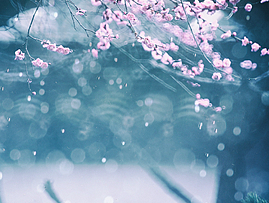
\includegraphics{test}
	
	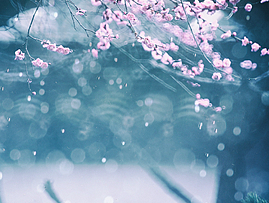
\includegraphics[scale=0.3]{test}
	
	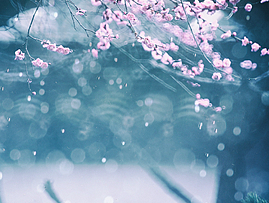
\includegraphics[height=2cm]{test}
	
	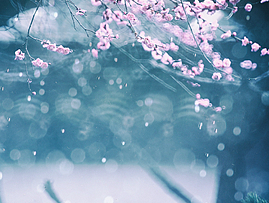
\includegraphics[height=0.1\textheight]{test} 	% \textheight整个页面的高度
	
	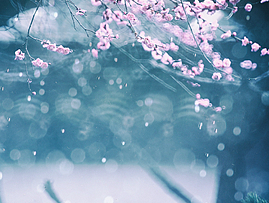
\includegraphics[width=0.2\textwidth]{test}		% \textwidth整个页面的宽度
	
	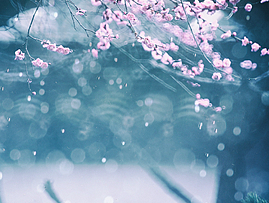
\includegraphics[width=\linewidth]{test}
	
	% ---------表格----------------
	\begin{tabular}{|l||p{1.5cm}|c|c r|} % l - 左对齐, c - 居中对齐, r - 右对齐, | - 竖线, p - 宽度
		\hline	% 横线
		类型 & 耕地 & 草地 & 林地 & 荒地 \\
		\hline \hline % 双横线
		A村 & 23 & 435 & 23 & 53 \\
		\hline
		B村 & 42 & 3234 & 76 & 5 \\
		\hline
	\end{tabular}

	% 三线表格, booktab longtab - 跨页长表格, tabu 综合表格
	% texdoc booktab
	% texdoc longtab
	% texdoc tabu
	
	% ---------浮动体环境----------------
	\LaTeX 中的插图与交叉引用:图\ref{fig-image} 图\ref{fig-image2}
	\begin{figure}[htbp]
		\centering % 居中
		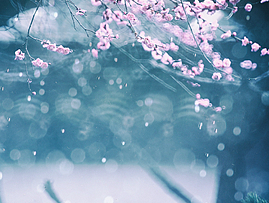
\includegraphics[height=2cm]{test}
		\caption{\TeX 哈哈哈} \label{fig-image}
	\end{figure}

	\begin{figure}[htbp]
	\centering % 居中
	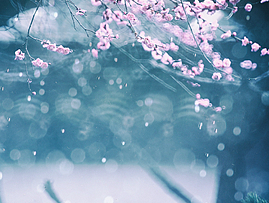
\includegraphics[height=2cm]{test}
	\caption{\TeX 哈哈哈} \label{fig-image2}
	\end{figure}

	% 允许位置: 默认为tbp
	%	h - here此处
	%	t - top页顶
	%	b - bottom页底
	%	p - page 独立一页


	\LaTeX 中的表格与交叉引用:表\ref{fig-tab}
	\begin{table}
		\centering % 居中
		\begin{tabular}{|l||p{1.5cm}|c|c r|} % l - 左对齐, c - 居中对齐, r - 右对齐, | - 竖线, p - 宽度
			\hline	% 横线
			类型 & 耕地 & 草地 & 林地 & 荒地 \\
			\hline \hline % 双横线
			A村 & 23 & 435 & 23 & 53 \\
			\hline
			B村 & 42 & 3234 & 76 & 5 \\
			\hline
		\end{tabular}
		\caption{\TeX 哈哈哈} \label{fig-tab}
	\end{table}
	
	
	% 标题控制宏包		caption bicaption
	% 并排和子图表宏包		subcaption subfig floatrow
	% 绕排宏包			picinpar wrapfig
	
	% ---------数学模式 $$-------------
	% 数学模式外面都是文本模式
	Let $f(x)$ be the defined by the formula.
	
	% 行内公式
	$f(x)=3x^2+x-1$.
	
	\(f(x)=3x^2+x-1\).
	
	\begin{math}
		f(x)=3x^2+x-1
	\end{math}
	
	% 上标和下标
	\begin{math}
	3x^y,x^{20},x^{2^3+m},a_0,a_{20}
	\end{math}
	
	% 希腊字母
	$\alpha^2$
	$\beta_a$
	$\gamma$
	$\epsilon$
	$\pi$
	$\omega$
	
	$\Gamma$
	$\Delta$
	$\Theta$
	$\Pi$
	$\Omega$
	
	% 数学函数
	$\sin \cos \log \arcsin \ln$
	
	$\ln 2$
	
	$\sqrt{\ln 2}$
	
	$\sqrt[4]{\ln 2}$
	
	$\frac{3}{4}$
	
	$\frac abc$
	
	% 行间公式
	$$f(x)=3x^2+x-1$$.
	
	\[f(x)=3x^2+x-1\].
	
	\begin{displaymath}
		f(x)=3x^2+x-1
	\end{displaymath}
	
	对于直角三角形$ABC$, 其中 $\angle C=90\degree$,则有
	% equation环境可以生成带有编号的行间公式.
	\begin{equation}
	AB^2 = BC^2 + AC^2	\label{eq:com1}
	\end{equation}
	
	\begin{equation*}	% 没有编号, 需要\usepackage{amsmath}
		a=b	\label{eq:com2}
	\end{equation*}
	
	
	如公式\ref{eq:com1}所示。
	
	% 多行数学公式
	% 需要 \usepackage{amsmath}
	% 	和 \usepackage{amssymb}
	\begin{gather}
		a+b=b+a\\
		ab=ba
	\end{gather}
	
	\begin{gather*}
		a\times b=b \times a\\
		a*b=b*a
	\end{gather*}
	
	\begin{gather}
		a+b=b+a \notag \\	% \notag阻止编号
		ab=ba
	\end{gather}
	
	\begin{align}	% 在&处对齐
		x &= 2y+z	\\
		2x &= 4y
	\end{align}
	
	\begin{align*}
		x &= 2y+z	\\
		2x &= 4y
	\end{align*}
	
	\begin{equation}
		\begin{split}	% 一个公式的多行排版
			x &= 2y+z	\\
			&= 4y
		\end{split}
	\end{equation}
	
	\begin{equation}
	\begin{split}	% 分段公式
	x =\begin{cases}
	1, & \text{如果 } x \in \mathbb{Q}; \\
	2, & \text{如果 } x \in \mathbb{R}\setminus\mathbb{Q}.
	\end{cases}
	\end{split}
	\end{equation}
	
	% 矩阵
	% 需要\usepackage{amsmath}
	% 常用的省略号 \dots \vdots \ddots 
	\[
		\begin{matrix}
		1 & 1 \\
		3 & 4
		\end{matrix}
		\begin{pmatrix}
		1 & 1 \\
		3 & 4
		\end{pmatrix}
		\begin{bmatrix}
		1 & 1 \\
		3 & 4
		\end{bmatrix}
		\begin{Bmatrix}
		1 & 1 \\
		3 & 4
		\end{Bmatrix}
		\begin{vmatrix}
		\text{\large 1} & 1 \\	% 临时切换text环境,改变字体大小
		3 & 4
		\end{vmatrix}
		\begin{Vmatrix}
		1 & 1 \\
		3 & 4
		\end{Vmatrix}
		\begin{Vmatrix}
		\dots & \vdots \\
		\ddots & \adots	% \adots是由\newcommand的定义
		\end{Vmatrix}
		\left(%
		\begin{smallmatrix}	% 行内小矩阵
		1 & 1 \\
		3 & 4
		\end{smallmatrix}
		\right)%
	\]
	
	% array 环境 - 和tabular环境很类似
	% array 环境可以排版更为复杂的矩阵
	\[
	\begin{array}{r|r}
	2 & 4\\
	\hline
	3 & f
	\end{array}
	\]
	
	
	% 文献管理:bib-------------------------------
	% bib自己布置参考文献 - 麻烦,不推荐使用。
	% cite{aritcle1}
	\if false 
	\begin{thebibliography}{99}
		
	\end{thebibliography}
	\fi 
	
	% 文献管理:Bibtex-------------------------------
	\if false
	% 使用Bibtex
	我来引用一下:\cite{Jr2006A,银温泉2001我国地方市场分割的成因和治理}
	
	引用一下才会下面的参考文献中显示:
	
	
	% 不引用,数据库全部文献列在下方
	% \nocite{*}
	\bibliography{ref}
	% 多个数据库
	% \bibliography{ref, cnki}
	\fi
	
	% 文献管理:Biblatex-------------------------------
	% biblatex/ biber 是新的tex参考文献排版引擎。
	% biblatex的样式文件制作简单,采用latex编写:bbx:参考文献样式文件, cbx:引用样式文件
	% 支持根据本地化排版
	% biber -l zh__pinyin texfile % 按照拼音进行排序
	% biber -l zh__stroke texfile % 按照笔画进行排序
	无格式化引用 \cite{aa}

	带方括号的引用 \parencite{aa}
	
	上标引用 \supercite{aa}
	
	% \nocite{*}
	\printbibliography[title={参考文献}]
	
\end{document}